%%%%%%%%%%%%%%%%%%%%%%%%%%%%%%%%%%%%%%%%%%%%%%
%Data Scientist for  Day - Codelab tutorial

%Copyright (C) 2013  Ferrari Alessandro

%This program is free software: you can redistribute it and/or modify
%it under the terms of the GNU General Public License as published by
%the Free Software Foundation, either version 3 of the License, or
%(at your option) any later version.

%This program is distributed in the hope that it will be useful,
%but WITHOUT ANY WARRANTY; without even the implied warranty of
%MERCHANTABILITY or FITNESS FOR A PARTICULAR PURPOSE.  See the
%GNU General Public License for more details.

%You should have received a copy of the GNU General Public License
%along with this program.  If not, see <http://www.gnu.org/licenses/>.
%%%%%%%%%%%%%%%%%%%%%%%%%%%%%%%%%%%%%%%%%%%%%%
\documentclass[aps,letterpaper,10pt]{revtex4}
\input kvmacros % For Karnaugh Maps (K-Maps)

\usepackage{graphicx} % For images
\usepackage{float}    % For tables and other floats
\usepackage{verbatim} % For comments and other
\usepackage{amsmath}  % For math
\usepackage{amssymb}  % For more math
\usepackage{fullpage} % Set margins and place page numbers at bottom center
\usepackage{listings} % For source code
\usepackage{subfig}   % For subfigures
\usepackage[usenames,dvipsnames]{color} % For colors and names
\usepackage[pdftex]{hyperref}           % For hyperlinks and indexing the PDF
\usepackage{tikz}
\usetikzlibrary{shapes,snakes}
\hypersetup{ % play with the different link colors here
    colorlinks,
    citecolor=blue,
    filecolor=blue,
    linkcolor=blue,
    urlcolor=blue % set to black to prevent printing blue links
}

\definecolor{mygrey}{gray}{.96} % Light Grey
\lstset{ 
	language=[ISO]C++,              % choose the language of the code ("language=Verilog" is popular as well)
   tabsize=4,							  % sets the size of the tabs in spaces (1 Tab is replaced with 3 spaces)
	basicstyle=\tiny,               % the size of the fonts that are used for the code
	numbers=left,                   % where to put the line-numbers
	numberstyle=\tiny,              % the size of the fonts that are used for the line-numbers
	stepnumber=2,                   % the step between two line-numbers. If it's 1 each line will be numbered
	numbersep=5pt,                  % how far the line-numbers are from the code
	backgroundcolor=\color{mygrey}, % choose the background color. You must add \usepackage{color}
	%showspaces=false,              % show spaces adding particular underscores
	%showstringspaces=false,        % underline spaces within strings
	%showtabs=false,                % show tabs within strings adding particular underscores
	frame=single,	                 % adds a frame around the code
	tabsize=3,	                    % sets default tabsize to 2 spaces
	captionpos=b,                   % sets the caption-position to bottom
	breaklines=true,                % sets automatic line breaking
	breakatwhitespace=false,        % sets if automatic breaks should only happen at whitespace
	%escapeinside={\%*}{*)},        % if you want to add a comment within your code
	commentstyle=\color{BrickRed}   % sets the comment style
}

% Make units a little nicer looking and faster to type
\newcommand{\Hz}{\textsl{Hz}}
\newcommand{\KHz}{\textsl{KHz}}
\newcommand{\MHz}{\textsl{MHz}}
\newcommand{\GHz}{\textsl{GHz}}
\newcommand{\ns}{\textsl{ns}}
\newcommand{\ms}{\textsl{ms}}
\newcommand{\s}{\textsl{s}}



% TITLE PAGE CONTENT %%%%%%%%%%%%%%%%%%%%%%%%
% Remember to fill this section out for each
% lab write-up.
%%%%%%%%%%%%%%%%%%%%%%%%%%%%%%%%%%%%%%%%%%%%%
\newcommand{\labtitle}{Data Scientist for a Day}
\newcommand{\authorname}{Alessandro Ferrari}
\newcommand{\emailauthor}{alessandroferrari87@gmail.com}
\newcommand{\classno}{Remote Sensing}
\newcommand{\professor}{Prof. Alberto Signoroni}
\newcommand{\university}{Universit\'a degli Studi di Brescia}
\newcommand{\presentationdate}{18 December 2013, Brescia}
% END TITLE PAGE CONTENT %%%%%%%%%%%%%%%%%%%%


\begin{document}  % START THE DOCUMENT!


% TITLE PAGE %%%%%%%%%%%%%%%%%%%%%%%%%%%%%%%%%%%%%%
% If you'd like to change the content of this,
% do it in the "TITLE PAGE CONTENT" directly above
% this message
%%%%%%%%%%%%%%%%%%%%%%%%%%%%%%%%%%%%%%%%%%%%%%%%%%%
\begin{titlepage}
\begin{center}
{\Large \textsc{\labtitle} \\ \vspace{4pt}} 
\rule[13pt]{\textwidth}{1pt} \\ \vspace{150pt}
{\large author: \authorname \\ \vspace{10pt}
email: \emailauthor \\ \vspace{10pt}}
\end{center}
\end{titlepage}
% END TITLE PAGE %%%%%%%%%%%%%%%%%%%%%%%%%%%%%%%%%%


%%%%%%%%%%%%%%%%%%%%%%%%%%%%%%
%%%%%%%%%%%%%%%%%%%%%%%%%%%%%%
\section{Introduction}
Today, the codelab will guide you through the effective application of a really powerful classification algorithm, the Support Vectors Machine, a.k.a. SVM. To make things more enganging, the lab session is contextualized in a Kaggle competition, the London Data Science competition. Have you ever heard about \href{www.kaggle.com}{Kaggle}? It is the place where world class data scientists compete. If you make it through until the end of the lab, you will be able to make your submission and to show up in the Kaggle leaderboard. Do not expect to be in the top straightaway from the first submission, you will have to face the best data scientists in the world. However, if you keep studying and improve your machine learner skills, we may see you soon among the top ones.

You probably know many theorical stuffs about classifiers, and you may be really good in showing off a lot of acronymous such as SVM, KNN, ANN and so on, however, you may feel as I did when I first approached the application of a classification task. You may think about which kind of classifier is better to apply for your challenge, or you may like to try an SVM as the first try but without any clue on the type of kernel that you have to choose, and ... what about the parameters ?!? The default ones do not look to work at all, right? If you are curious about the conclusion of this story, stay in tune with the lab, you will get some answers.

The dataset is the original one from the kaggle website. It is a synthetically generated dataset, I personally think that is a great playground for tuning and improve the effectiveness of classification solutions.

Enjoy!

\section{Instruction to the use of this lab}
As usual, few words before to proceed with the cool stuffs. If you are not acquainted with concepts such as basic fundamentals of machine learning, statistical metrics, model selection, learning curves and so on, I strongly recommend you to read in advance the lab track the day before the practical session. For timing issues, it will not be possible to cover both the theorical part and the practical part in the workshop. Even if you have not a strong background on those stuffs and some of the terms and notations will look obscure, I am sure you can finish the lab session. Machine learning is successful because is really practical, so you can use the presented instruments as black boxes. However, a theorical understanding will let you catch some details and reach a deeper understanding, that can help you to improve your results.

Be sure to have a python environment correctly configured on your computer. I suggest you to have a python IDE for developing the code of the lab. You may not necessarily need it, if you are good enough with the command line, however if you are not one of those kind of vintage-lovers, Eclipse with the PyDev plugin can be a good solution, Aptana can be an equivalent alternative.
For installing python modules, it is really useful to setup easy{\_}install for installing new modules. Windows user may take a look \href{http://simpledeveloper.com/how-to-install-easy{\_}install/}{here}, while linux user may simply type in their command line "sudo apt-get install python-setuptools". 
During the labs numpy, matplotlib and scikit-learn modules are required, you may think about to install them in advance with easy{\_}install.

By this lab, you can learn many precious stuffs that can make the difference in your professional career as a technology professional. When you do things actively you can memorize also ten times more, so make yourself a gift, be active! There are few rules that you need to follow:
\begin{itemize}
\item Do you have numpy, matplotlib and scikit-learn documentation websites open? If you do not, I will not help you.
\item Did your lab mate ask you a question without having opened the numpy, matplotlib and scikit-learn  documentation websites? Do not help him/her.
\item Are you having troubles on finding numpy documentation online? Click  \href{http://lmgtfy.com/?q=numpy+doc}{here}. For how concern matplotlib click \href{http://lmgtfy.com/?q=matplotlib}{here} and for how concern scikit-learn click \href{http://lmgtfy.com/?q=scikit-learn}{here}.
\item{You will find the code of the lab in the source folder, you have to complete some functions in order to make it work. Try to understand the different topics and then get involved in the exercises so that you can apply what you have learnt.}
\item{Be active.}
\item{If you score better than I did in the Kaggle competition, you have to tell me how you did it!}
\item{Enjoy!}
\item{Please, send me feedback to improve the laboratory for next years.}
\end{itemize}
Are you ready? Let's go!

\section{Introduction to Machine Learning}
\subsection{Few very brief general concepts}
Supervised Learning is a branch of machine learning that studies identification of complex functions by analysis of labeled or continuously valued data, that are also referred as training data. The training data are a series of examples; each example consists of a features vector and the corresponding label, in case a classification function has to be identified, conversely if it is a regression problem, instead of labels there are continuous values. Classification is the task to predict classes to which certain data belong. The classification function, also referred as classifier or as hypothesis, is the result of the supervised learning algorithm. Conversely, regression problems have the aim to identify a regression function in order to predict continuous value functions. 

In this codelab, just classification algorithms will be taken in analysis. The development of a classification algorithm is composed by two different phases, the learning phase, where the classification function is learned from the training set, and the classification phase, where the learned classification function is used to infer the labels for new features vectors received in input.

There are several different classification algorithms available. While the number of training samples increases, the performance of those algorithms asynthotically tend to be equivalent. However, in certain conditions, there are certain algorithms that are more suitable than others. Some algorithms are faster than others, some others have better learning in conditions of low-dimensionality of the training set, while certain others can achieve better classification rates but they are effective only in conditions of high dimensionality of the training set.

\subsection{Support Vector Machines}
The Support Vector Machine algorithm is a very powerful classification algorithm, that is widely used in industrial and academical applications. SVM is designed in a way that allows a fast and efficient integration with kernel-based techniques, so in certain conditions it may give a cleaner and faster way for learning complex nonlinear functions, compared to other state-of-the-art algorithms such as neural networks or logistic regression. The way how the SVM cost function is defined allows very efficient solutions as a convex optimization problem; this can guarantee great performance in several different conditions. When SVM is applied using kernel methods, it can be considered fast until when the training set dimensionality does not become too big (indicatively, the training set should be smaller than 100000 examples). The achieved level of optimization is a result coming from a long effort of the research community. Still, this optimizations may be insufficient in case of a really big training set dimensionality, in such cases you may evaluate to use a neural network.

SVM may be used as a linear classifier, if used without kernel methods, however in this lab session it will be used to learn a nonlinear decision boundary, so it will be applied with kernel methods. In general, if a sufficient number of training samples is available and there is not a priori knowledge about the characteristics of the hypothesis function that has to be learnt, it is suggested to apply SVM with radial basis functions kernel, also known as gaussian kernel. Unless it is known that the samples belonging to different classes are linearly separable, or unless the number of training samples is very low, there are not many reasons that suggest to use SVM without kernels. Today in the lab, SVM with gaussian kernels has been adopted. The gaussian kernel requires as a parameter the sigma of the "gaussian similarity function", it will be seen later on how the selection of this parameter is important in order to have good classification results. SVM has been chosen between all the different algorithms because it is expected to be easier to train, faster in the convergence of the learning phase, faster in the classification phase, flexible to the different distributions that may occur in the features space and it does not risk to get stuck in local minimum in the optimization problem like it may happens for some other algorithms.

\subsection{High Bias vs High Variance}
As anticipated beforehand, the SVM algorithm with gaussian kernels has an important parameter that has to be set, that is the sigma of the gaussian kernels. Smaller values of sigma corresponds to narrower kernel basis functions, that allows the algorithm to learn more complex wiggled curves. Conversely the bigger the values of sigma, the more regular and the simpler will be the learnt hypothesis. 

One may think that is always better to have an algorithm able to learn an as much complicated as possible hypothesis in order to achieve the best performances. This is indeed wrong, since sometimes the hypothesis that we have to learn are just regular. If it is attempted to fit a very complex model to a set of data that requires just a pretty regular decision boundary, in absence of a "sufficiently huge" amount of data, the hypothesis will probably suffer from overfitting or high variance (Fig.1). In this case it will be obtained a really wiggly decision boundary that will fit perfectly the training set and will guarantee very low training error, however it will generalize badly on new examples. As it is possible to see in Fig.1, the data are placed in a 2D features space in a way that suggests to separate them by a quadratic decision boundary, however since the data have been trained using an SVM with a very small sigma value, the decision boundary obtained is way more complicated and it is expected that will perform badly in the classification of new examples placed close to the boundary region. 

In Fig.2 it is shown how the data are fitted with a better choice of the sigma parameter, the
decision boundary is regular, it fits well the data and it is expected that the designed hypothesis will generalize well on new examples. So the choice of sigma is just fine. 

Conversely, in Fig.3 it is shown the opposite situation that may arise when fitting the data with a sigma parameters that is too big. The model that has been fitted to the data is not just a good model in order to separate the data. In fact the model is too regular and it will not be able to adapt to the dynamics of the training examples. This situation is called underfitting or high bias. 

In order to fix overfitting, the first thing to do is to verify to have chosen a good value of the sigma parameter by means of model selection, to fit a good model to the data. If it has been done a good choice and still overfitting persists, the number of features should be reduced and regularization techniques should be adopted. If overfitting persists even after that all these strategies have been tried out, it is suggested to collect more data. In fact, the bigger the number of training samples, the more the overfitting is unlikely to occur in overfitting problems. Conversely, if underfitting problem occurs, it has to be addressed by trying to fit a more complex model to the training set, reducing the sigma parameter. The second operation to do in order to remove underfitting is to increase the number of features by finding out new and more discriminative features for describe data.

\begin{figure}[]
\minipage{0.32\textwidth}
  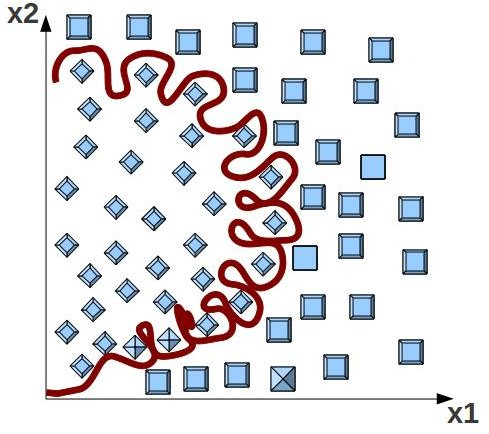
\includegraphics[width=\linewidth]{img/template_quadratic_region_overfitting.jpg}
  \caption{Decision boundary suffering of overfitting.}\label{fig:1}
\endminipage\hfill
\minipage{0.32\textwidth}
  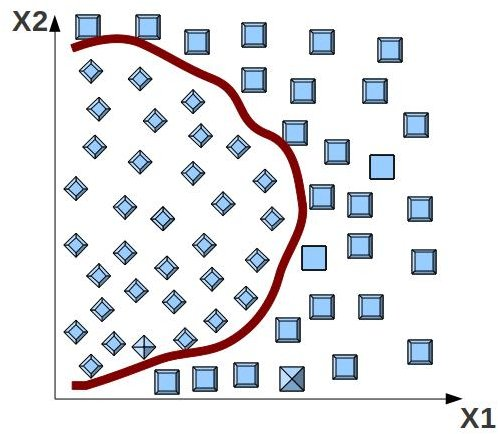
\includegraphics[width=\linewidth]{img/template_quadratic_region_just_right.jpg}
  \caption{Correctly regular decision boundary}\label{fig:2}
\endminipage\hfill
\minipage{0.32\textwidth}%
  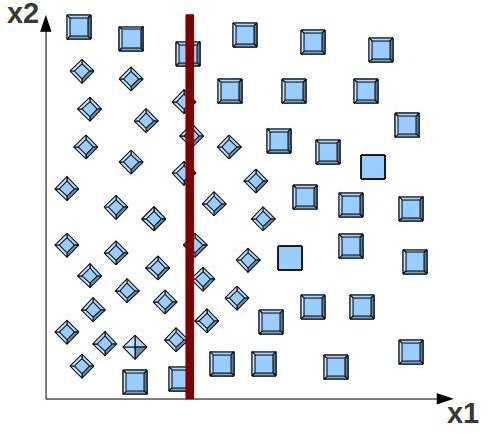
\includegraphics[width=\linewidth]{img/template_quadratic_region_underfitting.jpg}
  \caption{Decision boundary suffering of underfitting}\label{fig:3}
\endminipage
\end{figure}

\section{Stop chatting about classification... Let us classify!}
\subsection{Features Scaling}
In the learning phase of a classification algorithm, the hypothesis function that minimizes a certain cost function, that may vary depending on the algorithm that is selected, is searched. So, there is a search of the global minimum of the cost function relatively to that features space.  It is reasonable to assume that if features have ranges of different order of magnitude, the resulting features space will be really skewed and this may lead to several undesired counter effects. In order to avoid that the search of the global minimum follows complicated and slow paths, it is important to perform features scaling, all the features need to have reasonably similar ranges, in order to make more regular the features space. In fact, optimization operations work better in a smoother and more regular features space, and features scaling may help in achieving so.

\subsection{Hypothesis evaluation}
In the previous section, the hypothesis has been evaluated by means of observations at plots of a 2D features space. To look at plots is a very powerful and intuitive tools in order to understand how good a certain hypothesis is. However, to plot features spaces is not always possible, since they may assume very high-dimensionality. So, more general methods have been developed in order to evaluate how good a certain learnt hypothesis is. As it has already been anticipated, the training error, that is a measure of how well the hypothesis fits to the training set, is not a good way to evaluate if it has been obtained a good decision margin, since it may happen to have overfitting, so even if the training error is really low, the obtained hypothesis will generalize really bad to new examples. 

So, it is suggested to split the labeled dataset in two different subsets. The first subset will be used as a training set (70{\%} of the examples) while the second subset will used as a test set (30{\%} of the examples). The test set will be used to evaluate how the hypothesis, that has been designed by means of supervised learning on the training set, will generalize on new examples. In order to objectively evaluate performances, a measure of the classification performances has been defined, that is called the misclassification error measure. 

Misclassification measure can be computed because test examples are labeled with their correct classes, so that is possible to compare label inferred by the classifier with ground truth labels. For each classified example in the test set, if it has been classified correctly, 0 will be added to the error measure, while if it has been classified incorrectly,  will be added $1/m$ , with \textit{m} that is the total number of examples in the test set:
\begin{equation}
Err = \frac{1}{m_test}\sum_{i=1}^{m_test}incorrect( x_{i} )
\end{equation}
where \textit{incorrect} is a function that returns 1 if the example $x_{i}$ has been incorrectly classified,  it returns 0 otherwise.
This gives a measure of how well the learnt hypothesis will generalize on new examples.


% Define box and box title style
\tikzstyle{mybox} = [draw=red, fill=blue!20, very thick,
    rectangle, rounded corners, inner sep=10pt, inner ysep=20pt]
\tikzstyle{fancytitle} =[fill=red, text=white]

\begin{tikzpicture}
\node [mybox] (box){%
    \begin{minipage}{\textwidth}
        In the source folder of this codelab, you can find an incomplete implementation of the concepts explained in this lab track. You are supposed to understand the concepts and complete the code by your own. Once you have completed the code, for performing the classification of the dataset you have to run the main.py module. The main module calls some machine learning routines that are implemented in the classification.py module. In the first exercise you are supposed to implement the function misclassification\_errors in the classification.py module. Read carefully the comments that you find there and follows the indications that you received from the subsection above. P.s.: you can test your implementation only after that you have concluded also the next exercise!
    \end{minipage}
};
\node[fancytitle, right=10pt] at (box.north west) {Exercise 1};
\node[fancytitle, rounded corners] at (box.east) {$\clubsuit$};
\end{tikzpicture}%

\subsection{Error metrics for skewed classes}
Consider for instance that the problem of cancer classification is taken in analysis. Suppose that for each patients some features are extracted and these features well represent the clinical situation of the patient, so it is reasonable to think that will be possible to infer if the patient has the cancer by looking at them. After that learning has been done, it is obtained an algorithm that classifies correctly the 99\% of the examples in the test set. This sounds like a pretty remarkable achievement, however what was unsaid, it is that only the 1\% of the population have cancer. So, 99\% is the error rate that can be obtained by a dumb-classifier that predicts always that the patient has not cancer. The obtained algorithm does not look attractive anymore. 

In this case, it is said that there are skewed classes, this is common when positive samples occur very rarely. When we are analyzing such skewed classes is necessary to come up with different evaluation metrics. In particular, precision and recall metrics will be adopted. Let us us first present few definitions. Given a binary classification problem, it is defined as a true positive an example that is actually a positive and it is classified as a positive. It is defined as a true negative an example that is actually a negative and it is correctly classified as a negative. Then, it is defined as a false positive an example which its actual class is negative, but it is misclassified as a positive. Conversely, it is defined as a false negative an example that is actually positive and it is misclassified as negative. 

After that this bit notation has been introduced, it is possible to define the precision as following:
\begin{equation}
Precision= \frac{True positives}{True positives + False Positives}
\end{equation}
Recalling the previous example of cancer prediction, in case it is obtained a classifier with really high precision, if it is predicted that the patient has the cancer, there is a high probability that the patient actually has the cancer. So precision answers at the question: of all the patients that were predicted to have cancer, what fraction actually has the cancer? 

Now, another metric will be introduced in order to answer at the other question: of all patients that actually have cancer, what fraction did we correctly detect as having cancer? This metric is called recall and it is defined as following:
\begin{equation}
Recall = \frac{True positives}{True positives + False negatives}
\end{equation}
If it is obtained a classification algorithm with high recall, it is highly probable that the
cancer will be correctly detected to almost all the patients that actually have cancer.

Finally, we define a metric that attempt to give a measure of how good is our model in maximizing both precision and recall:
\begin{equation}
f1\_score = 2 * \frac{precision*recall}{precision+recall}
\end{equation}

\subsection{Model Selection}
In order to fit the correct model to the data, for avoiding overfitting and underfitting, it is important to select the best parameters. However, it has not yet been explained how to correctly select these parameters. In fact, the typical machine learning challenge does not have enough \textit{a priori} knowledge about the characteristics of the model that should be fitted. So, it has been necessary to develop a series of techniques in order to select the most suitable model, given the data. 

In the SVM classification algorithm with gaussian kernels, the parameters to set are the sigma of the gaussian kernel and the regularization constant. Regularization determines the regularity or smoothness of the obtained decision margin. The regularization constant is usually referred as C and it controls the strenght of regularization during the optimization process. It is a terrific tool to address overfitting. 

Now a question arises on how a good sigma parameter can be selected, so on how it can be selected the best model to fit the data. A set of possible different sigma and C values to evaluate is defined. So, let us say that is expected that the sigma parameters to be evaluated will be between the order of $10^{-7}$ and $10^{7}$ ; a set that starts with an element of value $10^{-7}$ and with the next elements that increase at logarithmic steps, until it is reached $10^{-7}$, such as {$10^{-7}$, $10^{-6}$, $10^{-5}$, $10^{-4}$,....,$10^{7}$}, is defined. The same applies for the regularization constant C, that will take value from a set with the same items as the sigma parameter. For each combination of these sigma and C parameters, the SVM training algorithm is applied on the training set. 

So, a hypothesis for each combination of the sigma and C parameters values is obtained. Then, the performances of all these hypothesis will be evaluated on the test set. The parameters corresponding to the hypothesis that will lead to the smallest classification error, will be selected as the best one. Once the best parameters are selected, to define new sets around the best values with higher resolution and to re-iterate model selection on the new sets can lead to a finer model selection. 

\begin{figure}[]
\minipage{0.32\textwidth}
  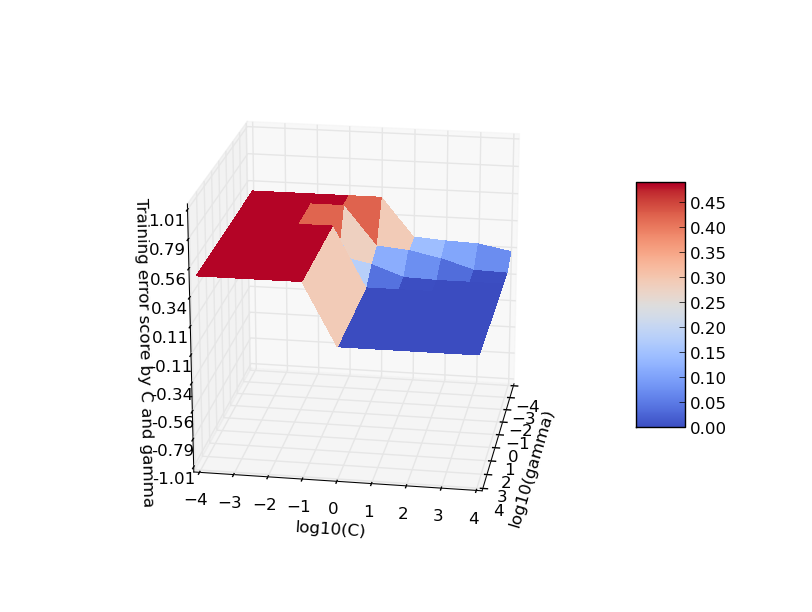
\includegraphics[width=\linewidth]{img/tr_err_graph.png}
  \caption{Training error plot of the model selection.}\label{fig:4}
\endminipage\hfill
\minipage{0.32\textwidth}
  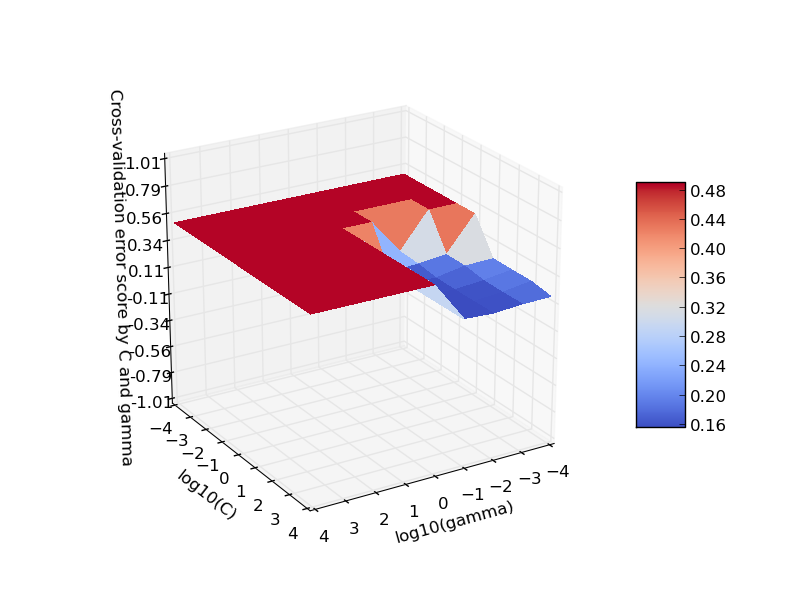
\includegraphics[width=\linewidth]{img/cv_err_graph.png}
  \caption{Cross-validation error plot of the model selection.}\label{fig:5}
\endminipage\hfill
\minipage{0.32\textwidth}%
  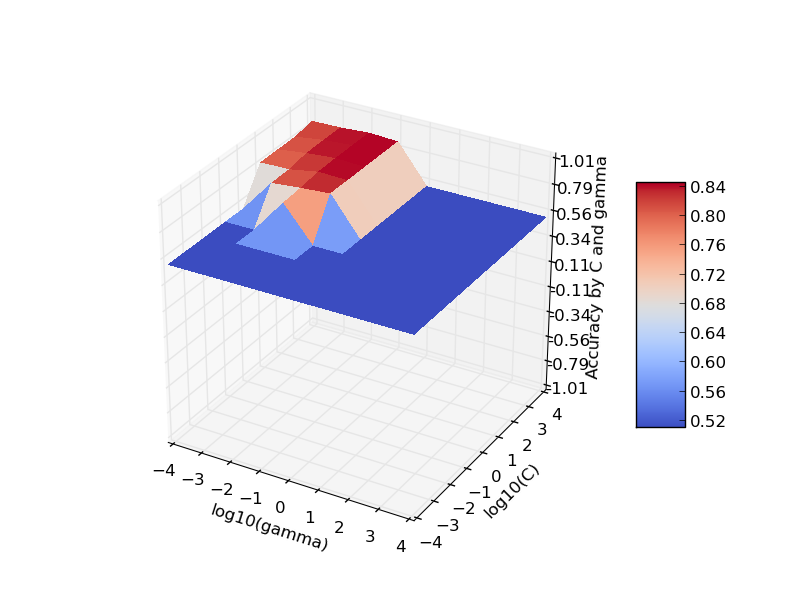
\includegraphics[width=\linewidth]{img/acc_graph.png}
  \caption{Accuracy plot of the model selection}\label{fig:6}
\endminipage
\end{figure}

\begin{figure}[]
\minipage{0.32\textwidth}
  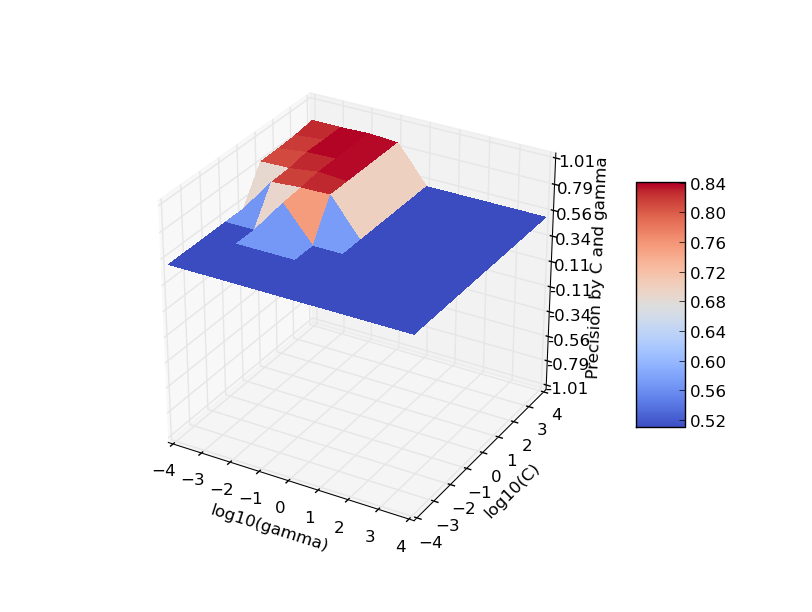
\includegraphics[width=\linewidth]{img/pr_graph.png}
  \caption{Precision plot of the model selection.}\label{fig:7}
\endminipage\hfill
\minipage{0.32\textwidth}
  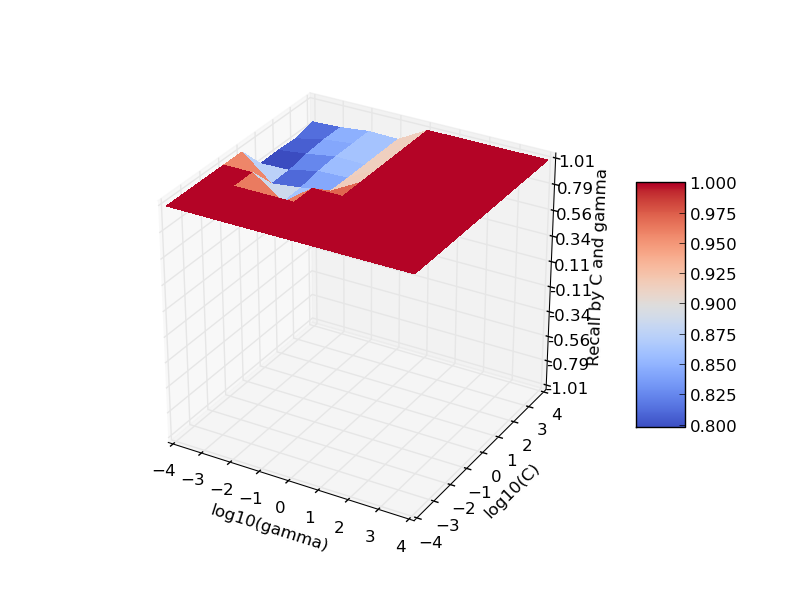
\includegraphics[width=\linewidth]{img/rec_graph.png}
  \caption{Recall plot of the model selection.}\label{fig:8}
\endminipage\hfill
\minipage{0.32\textwidth}%
  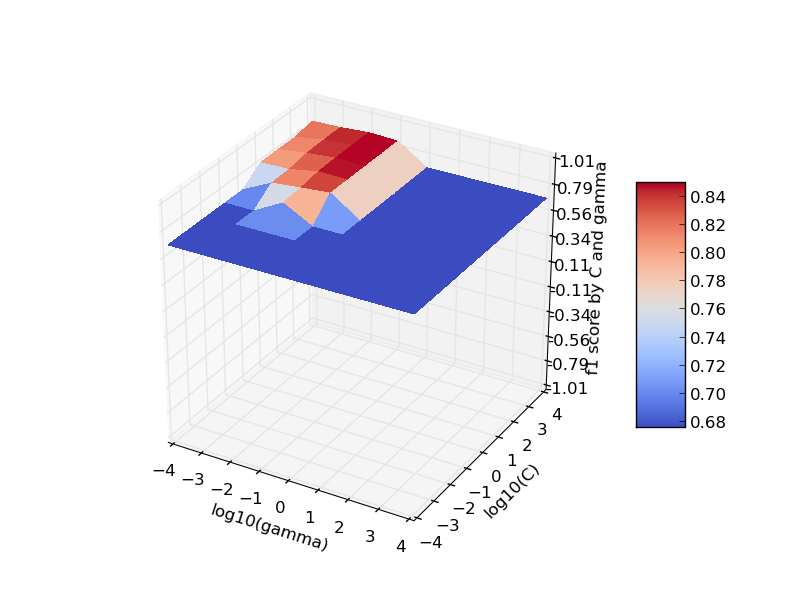
\includegraphics[width=\linewidth]{img/f1_graph.png}
  \caption{f1 plot of the model selection}\label{fig:9}
\endminipage
\end{figure}

\subsection{Dataset partitions re-arrangement}
In order to explain the following technique an example will be introduced first. Suppose that is desired to classify whether an object is a car or not. In the dataset there are a series of images of utility cars, sport cars and other objects. It is pretty much a fact that a desirable sport car does not look as ugly as a blend unemotional utility car. The sport car will be shorter in height, it will be longer and it will have several appearance differences compared to the utility car. Now, suppose also that the number of images with a utility car is way greater than the number of images with a sport car, that are just the 1\% of the objects in the dataset. It is desired that both utility cars and sport cars will be labeled as belonging to the category car. Let us say the dataset is partitioned in a training set with 70\% of the samples and a test set with the 30\% of the examples. 

Now, let us imagine that not even one of the images containing sport cars end up to be included in the training set, but they all end up in the test set. This will lead to a systematic error and all the sport cars in the test set will be classified as non-car objects, so it may be thought that the features chosen in order to classify sport cars are not good at all, however it may be a wrong conclusion, since there are not actual evidences that may measure how well the chosen features are in order to classify the sport cars. So, as it has been said before, sport cars may look fancier, thus it is not straightforward that the choice of features that will classify well utility cars, will have good performances on sport cars as well and suppose that is harder to have good classification performances on sport cars. 

Let us imagine the case where all the sport cars end up in the training set. The classification algorithm performs really well on utility cars and it is obtained a really high score in performances evaluation done on the test set. So, it will be expected that the designed algorithm will behave at the same way also on new examples. However, when new sport car examples will be classified, it may arise that the classifier is not effective on them since the features that have been chosen were insufficient, but this problem was not diagnosed in the algorithm debugging phase and so the right countermeasures have not been adopted in the algorithm design phase. 

In order to avoid to occur in a partitioning of the examples that leads to such unpleasant situations, several random partitions are extracted and for all of them the results of the classification algorithm are taken in analysis. If a sufficient number of partitions have been extracted, the worst results and the best results may be assumed as "reliable" boundaries of the performances that will be get when new examples will be examined. Moreover, by the gap between the worst and the best results, it is possible to understand how much our dataset suffers from the problems described above and it may be a hint that countermeasures should be adopted. In order to understand which countermeasures to adopt, is important to perform error analysis. Then by calculating the average of the results obtained on the different partitions, it is possible to understand whether the majority of the partitions give results that are closer to the better case or to the worst case. By averaging, a better performances evaluation is obtained.

% Define box and box title style
\tikzstyle{mybox} = [draw=red, fill=blue!20, very thick,
    rectangle, rounded corners, inner sep=10pt, inner ysep=20pt]
\tikzstyle{fancytitle} =[fill=red, text=white]

\begin{tikzpicture}
\node [mybox] (box){%
    \begin{minipage}{\textwidth}
        Now, you have all the necessary elements to complete the model selection code of the lab. You are supposed to have understood the concept of cross-validation for selecting the best parameters and the concept of dataset partitions re-arrangement for having robust statistics. Now, you can write the missing part of code in the method C\_gamma\_selection of the ModelSelection class, contained in the classification.py module. First understand the existing code and read carefully the comments, then implement your own part.
        
        Once you have finished the code of this exercise, look at the plots that you obtain from the model selection, which are the gamma and the C parameters that guarantee the best results? 
    \end{minipage}
};
\node[fancytitle, right=10pt] at (box.north west) {Exercise 2};
\node[fancytitle, rounded corners] at (box.east) {$\clubsuit$};
\end{tikzpicture}%

\subsection{Learning Curves}
Learning curves are often useful tools to diagnose whether a learning algorithm may be suffering from overfitting, underfitting or a bit of both. Beforehand let us introduce a bit  of notation. The  training error $J_{train}$ is the misclassification error measure applied to the training set, while the cross-validation error $J_{cv}$ is the misclassification error measure applied to the test set. In formulas:
\begin{equation}
J_{train} = \frac{1}{2m_{tr}} \sum_{i=1}^{m_{tr}}incorrect( x_i )
\end{equation}
\begin{equation}
J_{cv} = \frac{1}{2m_{cv}} \sum_{j=1}^{m_{cv}}incorrect( x_j )
\end{equation}
where $m_{tr}$ is the number of samples in the training set, $x^i$ is the features vector of the i-th example in the training set, $m_{cv}$ is the number of samples in the test set, $x_j$ is the features vector of the j-th example in the test set and incorrect is a function that gives 1 whether the example is misclassified, 0 whether is correctly classified.

In order to plot a learning curve, $J_{train}$ and $J_{cv}$ have to be draw as a function of the number of training examples. What has just been stated may result confusing, in fact the number of examples in a training set is a constant value. What was meant is to perform learning on a reduced training set, for instance starting from a 10 examples subset of the training set, calculate $J_{train}$ of the classifier obtained from the reduced training set and $J_{cv}$ on the complete test set, then iterate these steps while increasing the number of examples in the reduced training set, until the reduced training set corresponds to the entire training set.

When the training set is really small, like 10 examples, it is expected to have a really low
training error since the hypothesis can easily overfit the data, conversely it is expected a
really high cross-validation error, since very few samples have been encountered and so the
algorithm will not generalize well for new samples. As the number of samples in the
training set increases, the training error increases, since it becomes harder that the
hypothesis manages to fit all the training examples, while the cross-validation error
decreases, since it is reduced the overfitting and the decision region is better defined.

When the learning process has converged to an optimal decision boundary, it is expected that the training error and the cross-validation error converge to the same reasonably small error. In fact it is possible to empirically observe that the learning curves tend to flatten out as the number of examples increases. 

When an algorithm suffers from high bias, it is expected to have a high training error and a cross-validation error equivalent to the training error. In fact, with high bias, if new samples will be added, it is not expected that the decision boundary will change that much. If it is taken as example the case of underfitting shown in Fig.6.10, once the "best" possible straight line has been found (and it will be found pretty fast), adding new training examples will not change the decision boundary that will tend to stabilize, consequently the performances of the classifier will not change as well. The training error will be high and it will get constant relatively soon, since the decision boundary will stabilize relatively fast. For the same reason, if m is sufficiently large, the cross-validation error will be nearly equivalent to the training error, since the decision boundary will fit both sets at the same bad way. So, the learning curves of an algorithm suffering from high bias flatten out relatively soon and they flatten out at the same error value, as shown in Fig.10. 

Now the case when a learning algorithm suffers from high variance will be taken in analysis. In that case, it is expected that it relatively fits well the data and consequently the error on the training set will be small compared to the error obtained when the hypothesis generalizes to new examples. Thus, the learning curves of an algorithm in overfitting will have between $J_{train}$ and $J_{cv}$ the gap shown in Fig.12, that can be considered the diagnostic evidence of overfitting. By adding more data examples to the dataset is expected to reduce the gap and so to increase the performances of the learning algorithm. 

It is important to take into account that if a learning algorithm suffers from high bias, it is just a waste of time to collect more data, while in the case of overfitting, after that all the others tricks have been tried out, collect more data can actually improve performances.

% Define box and box title style
\tikzstyle{mybox} = [draw=red, fill=blue!20, very thick,
    rectangle, rounded corners, inner sep=10pt, inner ysep=20pt]
\tikzstyle{fancytitle} =[fill=red, text=white]

\begin{tikzpicture}
\node [mybox] (box){%
    \begin{minipage}{\textwidth}
        Finally, we are arrived at the last exercise. Soon, we will be able to make our Kaggle submission. This exercise, require that you have understood the concept of learning curves. Almost all the code necessary to implement learning curves have already been provided, however you need to understand it and you have to complete the last part. Read through carefully the code of the compute and StratifiedShuffleMask methods of the LearningCurves class in the classification.py module. First, understand the code of these methods, by using also the documentation of numpy and scikit-learn. Then, implement the missing part of the code following the indications in the comments. 
        
        After that the code is complete, you can run all the code until the plots of the learning curves. What do the learning curves suggest us? Is it suffering of underfitting, overfitting, or do you think it is fine?
        
        A new file predicted\_y.csv is produced by infering labels for the Kaggle test set features in the source folder. You can upload it in the Kaggle submission page of the London Data Science competition and see the score that you reached.  
    \end{minipage}
};
\node[fancytitle, right=10pt] at (box.north west) {Exercise 3};
\node[fancytitle, rounded corners] at (box.east) {$\clubsuit$};
\end{tikzpicture}%

\begin{figure}[]
\minipage{0.32\textwidth}
  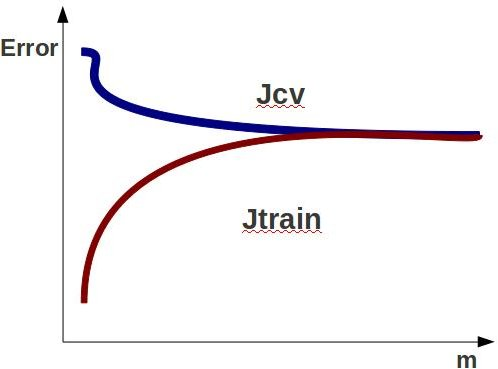
\includegraphics[width=\linewidth]{img/learning_curves_high_bias.jpg}
  \caption{Learning curves of an algorithm suffering of high bias.}\label{fig:10}
\endminipage\hfill
\minipage{0.32\textwidth}
  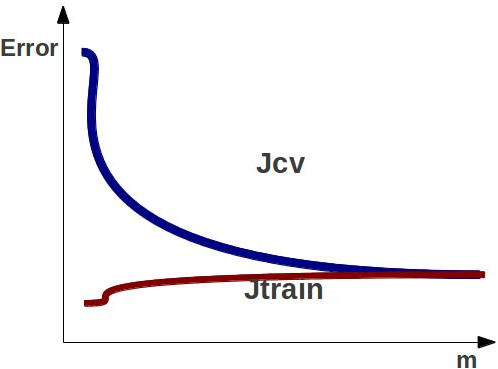
\includegraphics[width=\linewidth]{img/learning_curves_just_fine.jpg}
  \caption{Learning curves of an algorithm with good convergence.}\label{fig:11}
\endminipage\hfill
\minipage{0.32\textwidth}%
  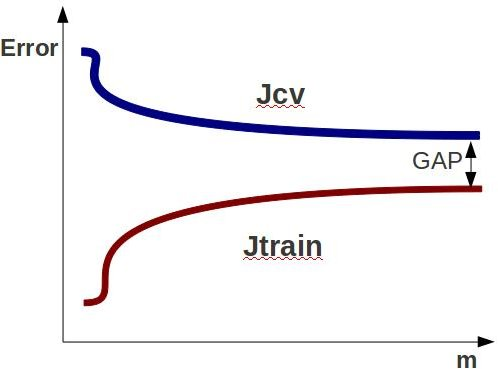
\includegraphics[width=\linewidth]{img/learning_curves_high_variance.jpg}
  \caption{Learning curves of an algorithm suffering of high variance.}\label{fig:12}
\endminipage
\end{figure}

\section{Conclusion}
If you have got through all the lab and you have understood all the concepts, you have reached a good starting level for applying machine learning tools. For improving your machine learner skills, I suggest you to follow the Machine Learning course of the Prof. Andrew Ng at www.coursera.org. In the scikit-learn website, you can find really interesting tutorials, that can be useful for improve your practical skills.

\section{License}
The copyright of this work is owned by the author, Alessandro Ferrari.
This work is licensed under the Creative Commons Attribution-ShareAlike 4.0 International License. To view a copy of this license, visit http://creativecommons.org/licenses/by-sa/4.0/.
\end{document} 